\documentclass[]{BasiliskReportMemo}
\usepackage{AVS}


\newcommand{\submiterInstitute}{Autonomous Vehicle Simulation (AVS) Laboratory,\\ University of Colorado}

\newcommand{\ModuleName}{test\textunderscore sunlineUKF}
\newcommand{\subject}{Sunline UKF Module and Test}
\newcommand{\status}{Initial document}
\newcommand{\preparer}{T. Teil}
\newcommand{\summary}{This module implements and tests a Unscented Kalman Filter in order to estimate the sunline direction.}


\begin{document}


\makeCover



%
%	enter the revision documentation here
%	to add more lines, copy the table entry and the \hline, and paste after the current entry.
%
\pagestyle{empty}
{\renewcommand{\arraystretch}{2}
\noindent
\begin{longtable}{|p{0.5in}|p{4.5in}|p{1.14in}|}
\hline
{\bfseries Rev}: & {\bfseries Change Description} & {\bfseries By} \\
\hline
Draft & Initial Revision & T. Teil \\
\hline

\end{longtable}
}

\newpage
\setcounter{page}{1}
\pagestyle{fancy}

\tableofcontents
~\\ \hrule ~\\

%\begin{figure}[htb]
%	\centerline{
%	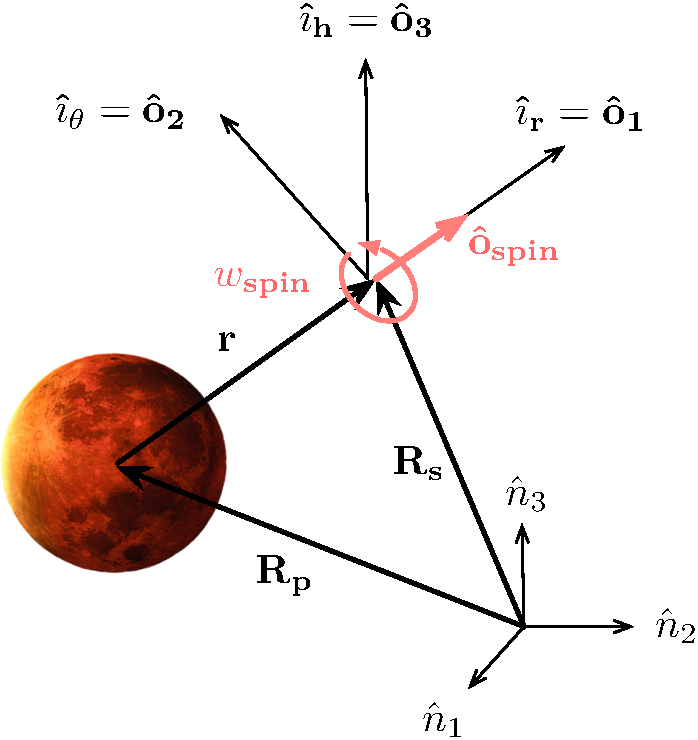
\includegraphics[]{Figures/Fig1}
%	}
%	\caption{Sample Figure Inclusion.}
%	\label{fig:Fig1}
%\end{figure}

\section{Introduction}
The Unscented Kalman filter (UKF) in the AVS Basilisk simulation is a sequential
filter implemented to give the best estimate of the desired states.
In this method we estimate the sun heading as well as it's rate of change along the observable axes.
The UKF reads in the message written by the coarse sun sensor, and writes a message 
containing the sun estimate. 

This document summarizes the content of the module, how to use it, and the test that 
was implemented for it. More information on the filter derivation can be found in Reference [\citenum{Teil:2018fe}], and more information on the square root unscented filter can be found in Reference [\citenum{Wan2001}] (attached alongside this document).


\subsection{Dynamics}

The states that are estimated in this filter are the sunline vector, and it's rate of change $\bm X^* = \begin{bmatrix} \bm d &  \dot{\bm d}\end{bmatrix}^T$. The star superscript represents that
this is the reference state. 

The dynamics are given in equation \ref{eq:dyn}. Given the nature of the filter, there is an unobservable state component: the rotation about the $\bm d$ axis. In order to remedy this, we project the states along this axis and subtract them, in order to measure only observable state components. 

\begin{equation}\label{eq:dyn}
\bm F(\bm X) = \begin{bmatrix} \bm F_1(\bm d) \\  \bm F_2(\dot{\bm d})\end{bmatrix} =  \begin{bmatrix} \dot{\bm d} - \left( (\bm d \cdot \dot{\bm d} )\frac{\bm d}{||\bm d||^2} \right) \\ - \frac{1}{\Delta t}\left( (\bm d \cdot \dot{\bm d}) \frac{\bm d}{||\bm d||^2} \right)\end{bmatrix} 
\end{equation}

The measurement model is given in equation \ref{eq:meas}, and the $H$ matrix defined as $H = \left[\frac{\partial \bm G (\bm X, t_i)}{\partial \bm X}\right]^{*}$ is given in equation $\ref{eq:Hmat}$. 

In this filter, the only measurements used are from the coarse sun sensor. For the $i^\mathrm{th}$ sensor, the measurement is simply given by the dot product of the sunline heading and the normal to the sensor. This yields easy partial derivatives for the H matrix, which is a matrix formed of the rows of transposed normal vectors (only for those which received a measurement). Hence the $H$ matrix has a changing size depending on the amount of measurements. 

\begin{equation}\label{eq:meas}
\bm G_i(\bm X) = \bm n_i \cdot \bm d
\end{equation}

\begin{equation}\label{eq:Hmat}
\bm H(\bm X) = \begin{bmatrix} \bm n_1^T \\ \vdots \\ \bm n_i^T \end{bmatrix} 
\end{equation}

\section{Filter Set-up, initialization, and I/O}

\subsection{User initialization}

In order for the filter to run, the user must set a few parameters:

\begin{itemize}
\item The unscented filter has 3 parameters that need to be set, and are best as: \\
      \texttt{ filterObject.alpha = 0.02} \\
      \texttt{ filterObject.beta = 2.0} \\
      \texttt{ filterObject.kappa = 0.0} 
\item The angle threshold under which the coarse sun sensors do not read the measurement: \\ 
\texttt{FilterContainer.sensorUseThresh = 0.}
\item The process noise matrix: \\
   \texttt{qNoiseIn = numpy.identity(5)} \\
   \texttt{ qNoiseIn[0:3, 0:3] = qNoiseIn[0:3, 0:3]*0.01*0.01} \\
   \texttt{ qNoiseIn[3:6, 3:6] = qNoiseIn[3:6, 3:6]*0.001*0.001} \\
    \texttt{filterObject.qNoise = qNoiseIn.reshape(25).tolist()}
\item The measurement noise value, for instance: \\
 \texttt{FilterContainer.qObsVal = 0.001}
\item The initial covariance: \\
 \texttt{Filter.covar =} \\
  \texttt{ [0.4, 0.0, 0.0, 0.0, 0.0, 0.0, \\
                          0.0, 0.4, 0.0, 0.0, 0.0, 0.0, \\
                          0.0, 0.0, 0.4, 0.0, 0.0, 0.0, \\
                          0.0, 0.0, 0.0, 0.04, 0.0, 0.0, \\
                          0.0, 0.0, 0.0, 0.0, 0.04, 0.0, \\
                          0.0, 0.0, 0.0, 0.0, 0.0, 0.04]}
\item The initial state :\\
 \texttt{Filter.state =[1.0, 0.0, 0.0, 0.0, 0.0, 0.0]}
\end{itemize}
The messages must also be set as such:

\begin{itemize}
\item    \texttt{ filterObject.navStateOutMsgName = "sunline$\_$state$\_$estimate"}
\item    \texttt{ filterObject.filtDataOutMsgName = "sunline$\_$filter$\_$data"}
\item   \texttt{ filterObject.cssDataInMsgName = "css$\_$sensors$\_$data"}
\item   \texttt{ filterObject.cssConfInMsgName = "css$\_$config$\_$data"}
\end{itemize}

\subsection{Inputs and Outputs}

The UKF reads in the measurements from the coarse sun sensors. These are under the form of a list of cosine values. Knowing the normals to each of the sensors, we can therefore use them to estimate sun heading.

\section{Test Design}
The unit test for the sunlineUKF module is located in:\\

\noindent
{\tt fswAlgorithms/attDetermination/sunlineUKF/$\_$UnitTest/test$\_$SunlineUKF.py} \\

As well as another python file containing plotting functions:

\noindent
{\tt fswAlgorithms/attDetermination/sunlineUKF/$\_$UnitTest/SunlineUKF$\_$test$\_$utilities.py} \\

The test is split up into 3 subtests. The first test creaks up all of the individual filter methods and tests them individually. These notably go over the square-root unscented filter specific functions. The second test verifies that in the case where the state is zeroed out from the start of the simulation, it remains at zero. The third test verifies the behavior of the time update with a measurement modification in the middle of the run. 

\subsection{Individual tests}

In each of these individual tests, random inputs are fed to the methods and their values are computed in parallel in python. These two values are then compared to assure that the correct computations are taking place. 
\begin{itemize}
\item \underline{QR Decomposition}: This tests the QR decomposition function which returns just the R matrix. Tolerance to error $\epsilon = 10^{-15}$.

\textcolor{ForestGreen}{Passed}
\item \underline{LU Decomposition}: This tests the LU Decomposition accuracy. Tolerance to error $\epsilon = 10^{-14}$.

\textcolor{ForestGreen}{Passed}
\item \underline{LU backsolve}: This tests the LU Back-Solve accuracy. Tolerance to error $\epsilon = 10^{-14}$.

\textcolor{ForestGreen}{Passed}
\item \underline{LU matrix inverse}: This tests the LU Matrix Inverse accuracy. Tolerance to error $\epsilon = 10^{-14}$.

\textcolor{ForestGreen}{Passed}
\item \underline{Cholesky decomposition}: This tests the Cholesky Matrix Decomposition accuracy. Tolerance to error $\epsilon = 10^{-14}$.

\textcolor{ForestGreen}{Passed}
\item \underline{L matrix inverse}: This tests the L Matrix Inverse accuracy. Tolerance to error $\epsilon = 10^{-14}$.

\textcolor{ForestGreen}{Passed}

\item \underline{U matrix inverse}: This tests the U Matrix Inverse accuracy. Tolerance to error $\epsilon = 10^{-12}$.

\textcolor{ForestGreen}{Passed}
\end{itemize}

\subsection{Static Propagation}


\input{AutoTeX/StatesPlotprop.tex}

This test also takes no measurements in, and propagates with the expectation of no change. It then tests that the states and covariance are as expected throughout the time of simulation. Plotted results are seen in Figure \ref{fig:StatesPlotprop}. We indeed see that the state and covariance that evolve nominally and without bias .

Tolerance to error: $\epsilon = 10^{-10}$

\subsection{Full Filter test}

This test the filter working from start to finish. No measurements are taken in for the first 20 time steps. Then a heading is given through the CSS message. Halfway through the simulation, measurements stop, and 20 time steps later a different heading is read. The filter must be robust and detect this change. This test is parametrized for different test lengths, different initial conditions, different measured headings, and with or without measurement noise. All these are successful.

\vspace{0.2cm}
Tolerance to error without measurement noise: $\epsilon = 10^{-10}$

\textcolor{ForestGreen}{Passed}

Plotted results are seen in Figures \ref{fig:StatesPlotupdate}, and \ref{fig:PostFitupdate}. Figure \ref{fig:StatesPlotupdate} shows the state error and covariance over the run. We see the covariance initially grow, then come down quickly as measurements are used. It grows once again as the measurements stop before bringing the state error back to zero with a change in sun heading. 

Figure \ref{fig:PostFitupdate} shows the post fit residuals for the filter, with no measurement noise. We see that the observations are read in well an that the residuals are brought back down to zero.

\input{AutoTeX/StatesPlotupdate.tex}
\input{AutoTeX/PostFitupdate.tex}


\bibliographystyle{AAS_publication}   % Number the references.
\bibliography{references}   % Use references.bib to resolve the labels.



\end{document}
